%!TEX encoding = UTF-8 Unicode
%!TEX TS-program = pdflatex

%%% --- PREAMBLE --- %%%
\documentclass[a4paper,11pt]{article}

\usepackage[italian]{babel}
\usepackage[left=2cm,right=2cm,top=2cm,bottom=2cm]{geometry}
\usepackage[T1]{fontenc} % OT1: basic, T1: western, T3 and T5: exotic, T4: lots of characters but WORSE READABILITY
\usepackage[utf8x]{inputenc} % utf8x supports more characters than utf8
\usepackage{graphicx} % import PNG, JPG and PDF with \includegraphics
\usepackage[usenames,table]{xcolor} % \color
\usepackage{amssymb}
\usepackage{amsmath}
\usepackage{amsfonts}
\usepackage{float}
\usepackage{mathtools} % (!! PLACE BEFORE hyperref !!)
\usepackage{xfrac} % \sfrac
\usepackage{cancel} % \cancel \cancelto
%\usepackage{hyperref} % interactive links in TOC, URLs and references
% unneded \usepackage{fixltx2e} % provides \textsubscript and makes some fixes
\usepackage[toc,page]{appendix}
\usepackage{siunitx} % \num \si \SI
\usepackage{alltt} % {alltt} (like verbatim but with commands)
\usepackage{moreverb} % {listing}
\usepackage{listings} % {lstlisting}
\usepackage[overload]{textcase} % fixes \MakeUppercase and \MakeLowercase
\usepackage[normalem]{ulem} % \uline \uwave \sout \xout
\usepackage{enumerate} % adds options for {enumerate}
\usepackage{paralist} % inline lists with {inparaenum}
\usepackage[official]{eurosym} % \euro
\usepackage{tabu} % {tabu} (like {tabular} with improvements)
\usepackage{layout} % layout description
\usepackage{multicol} % {multicols}
\usepackage{lipsum} % filling text generator with \lipsum
\usepackage[section]{placeins} % inhibits float figures from trepassing a section boundary
\usepackage{subfig} % \subfloat to be used inside {figure}
\usepackage{wrapfig} % {wrapfigure} (like {figure} but allows text to flow on its sides)
\usepackage{ifthen} % \ifthenelse
\usepackage{calc}
\usepackage{array}
\usepackage{multirow}
\usepackage{booktabs} % \toprule, \midrule, \bottomrule
\usepackage{fancyhdr}
\usepackage{wasysym}
\graphicspath{ {../Figs-Tabs/} } % graphics search directories
\setcounter{tocdepth}{1} % -1: part, 0: chapter, 1: section, 2: subsection, 3: subsubsection

\lstset{ %
	language=C,
	deletekeywords={},
	morekeywords={},
	backgroundcolor=\color{white},
	basicstyle=\ttfamily\small,
	commentstyle=\color{teal},
	keywordstyle=\color{magenta},
	stringstyle=\color{purple},
	identifierstyle=\color{violet!80!black},
	numbers=left,
	numbersep=7pt,
	numberstyle=\scriptsize\sffamily\color{gray},
	stepnumber=1,
	breakatwhitespace=false,
	breaklines=true,
	keepspaces=true,
	showspaces=false,
	showstringspaces=false,
	showtabs=false,
	tabsize=2,
	captionpos=none,
}

\newcommand{\swaphmargins}{
\newlength{\tmplength}
\setlength{\tmplength}{\oddsidemargin}
\setlength{\oddsidemargin}{\evensidemargin}
\setlength{\evensidemargin}{\tmplength}}

\newcommand{\setdispacing}[1][0pt]{\setlength{\abovedisplayskip}{#1}
\setlength{\belowdisplayskip}{#1}
\setlength{\abovedisplayshortskip}{#1}
\setlength{\belowdisplayshortskip}{#1}}

\newcommand{\inv}[1]{\frac{1}{#1}}
\newcommand{\dd}{\mathrm{d}}
\newcommand{\deriv}[2][x]{\frac{\dd #2}{\dd #1}}
\newcommand{\derivn}[3][x]{\frac{\dd^{#2}#3}{\dd{#1}^{#2}}}
\newcommand{\pardv}[2][x]{\frac{\partial #2}{\partial #1}}
\newcommand{\pardvn}[3][x]{\frac{\partial^{#2}#3}{\partial{#1}^{#2}}}
\newcommand{\integ}[2][x]{\int #2\,\dd #1}
\newcommand{\invinteg}[2][x]{\int\frac{\dd #1}{#2}}
\newcommand{\dinteg}[4]{\int_{#1}^{#2}#3\,\dd #4}
%\renewcommand{\arcsin}{\operatorname{asin}}
%\renewcommand{\arccos}{\operatorname{acos}}
%\renewcommand{\arctan}{\operatorname{atan}}
\DeclareMathOperator{\arccot}{arccot}
\newcommand{\vel}{\vee}
\newcommand{\et}{\wedge}

\newcommand{\fwhm}{\text{FWHM}}
\newcommand{\hwhm}{\text{HWHM}}

\newcommand{\ndr}[1]{\footnote{#1 (n.d.r.)}}
\newcommand{\fig}[1]{figura (\ref{f:#1})} %inserting reference to figures
\newcommand{\tab}[1]{tabella (\ref{t:#1})} % inserting reference to tables
\newcommand{\dof}{\text{ dof}} % degrees of freedom
\newcommand{\paral}{\mathbin{\|}} % impedance parallel
\DeclareSIUnit\deca{decade} % decade unit definition for use in siunitx

\newcommand{\insertpart}[2]{\input{#1}}
\newcommand{\e}{\textbf{$e^{-}$}}
\sisetup{%
	separate-uncertainty = true,
	per-mode = symbol,
	bracket-numbers = false,
	multi-part-units = single,
	table-number-alignment = center,
	range-phrase = \text{--},
	range-units = brackets,
	output-complex-root =  \text{\ensuremath{j}},
	table-figures-decimal = 4,
	table-figures-exponent = 0,
	table-figures-integer = 2,
	table-figures-uncertainty = 2,
}

%%% --- DOCUMENT --- %%%


%%%%% SIunitX example use:
% \si{\kilo\volt\per\meter\squared} -> kV/m^2
% \SI{1.222 (34)}{\joule\second}    -> 1.222 +- 0.034 Js
% \SI{1.222 \pm 0.034}{\nF}         -> 1.222 +- 0.034 nF
% use it plz
% ALSO the S tab column is pretty useful

\author{Gruppo BF \\ Thomas Giannoni, Valerio Lomanto, Roberto Ribatti}
\title{Esercitazione N.10: Caratteristiche delle porte logiche.}
\date{21 marzo 2017}
%Intestazione
\usepackage{fancyhdr}
\pagestyle{fancy}
\lhead{Esercitazione N.10}
\chead{caratteristiche fisiche delle porte logiche}
\rhead{Gruppo BF}
\begin{document}
\maketitle
\begin{abstract}
	L'obiettivo di questa esperienza è la misura di alcune delle caratteristiche delle porte NOT di un circuito integrato SN74LS04, verificando l'accordo tra le grandezze misurate e quelle fornite dal costruttore.
\end{abstract}

\section{Strumentazione}
La strumentazione usata è quella presente sul banco di lavoro,
		\begin{itemize}
			\item un circuito integrato SN74LS04 (hex inverter): le porte NOT da caratterizzare;
			\item un Arduino Nano, che servirà come sorgente di onde quadre;
			\item un circuito integrato SN74LS244 (buffer/driver), che ha la funzione di proteggere la scheda Arduino.
		\end{itemize}
Nel seguito tutte le misure dinamiche saranno eseguite con l'oscilloscopio, quelle statiche con il multimetro digitale, ad eccezione delle misure di piccole correnti che verranno eseguite con il multimetro analogico (più preciso in questo range).

\section{Caratteristiche statiche}
Il circuito integrato integrato SN74LS04 è alimentato ad una tensione $V_{cc} =\SI{5.01 \pm 0.03}{\volt}$.

\subsection{Misure delle tensioni d'operazione}
Si è montato il circuito in \figurename{ \ref{f:c1}}, dopodiché si è andati a  campionare la tensione in uscita $V_{out}$ in funzione della tensione di ingresso $V_{in}$.

\begin{figure}[H]
	\begin{minipage}{0.7\textwidth}
		\centering
		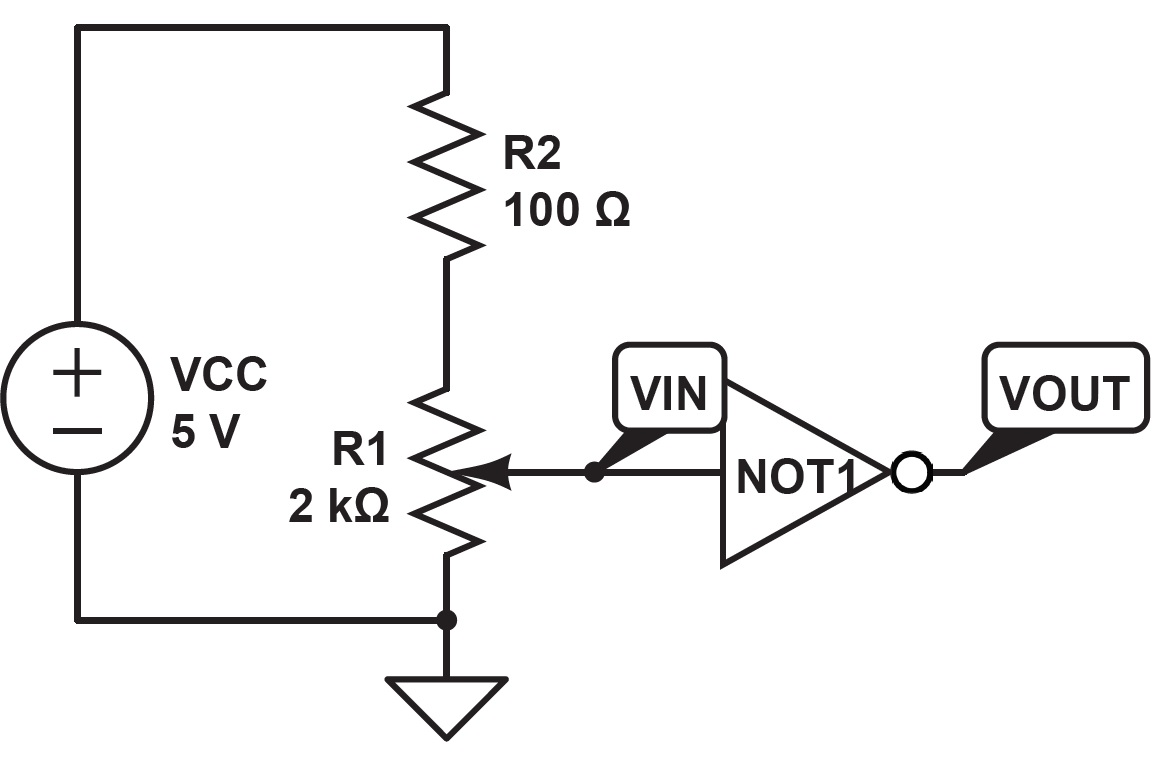
\includegraphics[width=0.7\textwidth]{immagine1.jpg}
		\caption{Circuito impiegato per lo studio delle tensioni d'operazione}
		\label{f:c1}
	\end{minipage}
	\begin{minipage}{0.3\textwidth}
		\begin{tabular}{l}
			$R_1 = \SI{1.993(18)}{\ohm}$\\
			$R_2 = \SI{100.8(9)}{\ohm}$
			%R1 me lo sono inventato, alla faccia vostra :p
		\end{tabular}
	\end{minipage}
\end{figure}

Si è variata la tensione in ingresso $V_{in}$ agendo sul trimmer $R_1$ e misurando la variazione della tensione in uscita $V_{out}$. I dati raccolti sono riportati in appendice in \tablename{ \ref{t:1}}.

In \figurename{ \ref{f:i1}} è riportato il grafico dei dati raccolti.
Siamo interessati ai seguenti parametri:
\begin{itemize}
\item $V_{IH}$ tensione in ingresso minima per cui  l'uscita è LOW (da datasheet < \SI{0.4}{\volt});
\item $V_{IL}$ tensione in ingresso massima per  l'uscita è HIGH (da datasheet > \SI{2.4}{\volt});
\item $V_{OH}$ tensione in uscita minima per cui l'ingresso è LOW (da datasheet < \SI{0.8}{\volt});
\item $V_{OL}$ tensione in uscita massima per cui  l'ingresso è HIGH (da datasheet > \SI{2}{\volt}).
\end{itemize}

Di seguito si riportano i valori misurati e i valori limite riportati nel datasheet:

\begin{table}[H]
	\centering
	\begin{tabular}{l l}
	$V_{IH}=$\SI{1.108(6)}{\volt} & $V_{IH}^{exp}=$\SI{2}{\volt}\\
	$V_{IL}=$\SI{1.003(6)}{\volt} & $V_{IL}^{exp}=$\SI{0.8}{\volt}\\
	$V_{OH}=$\SI{3.87(3)}{\volt} & $V_{OH}^{exp}=$\SI{2.4}{\volt}\\
	$V_{OL}=$\SI{172.7(9)}{\milli\volt} & $V_{OL}^{exp}=$\SI{0.4}{\volt}
\end{tabular}
\end{table}

I valori misurati sono migliori di quelli dichiarati, la differenza è dovuta al fatto che siano misurati nelle peggiori condizioni di operatività possibili della porta NOT.

Per tensioni compresa tra 	$V_{IL}$ ed $V_{IH}$ il segnale in uscita oscilla tra lo stato HIGH e LOW in maniera apparentemente casuale, del resto il comportamento del circuito in questo range non è stabilito.

\begin{center}
	\begin{figure}[H]
		\centering
		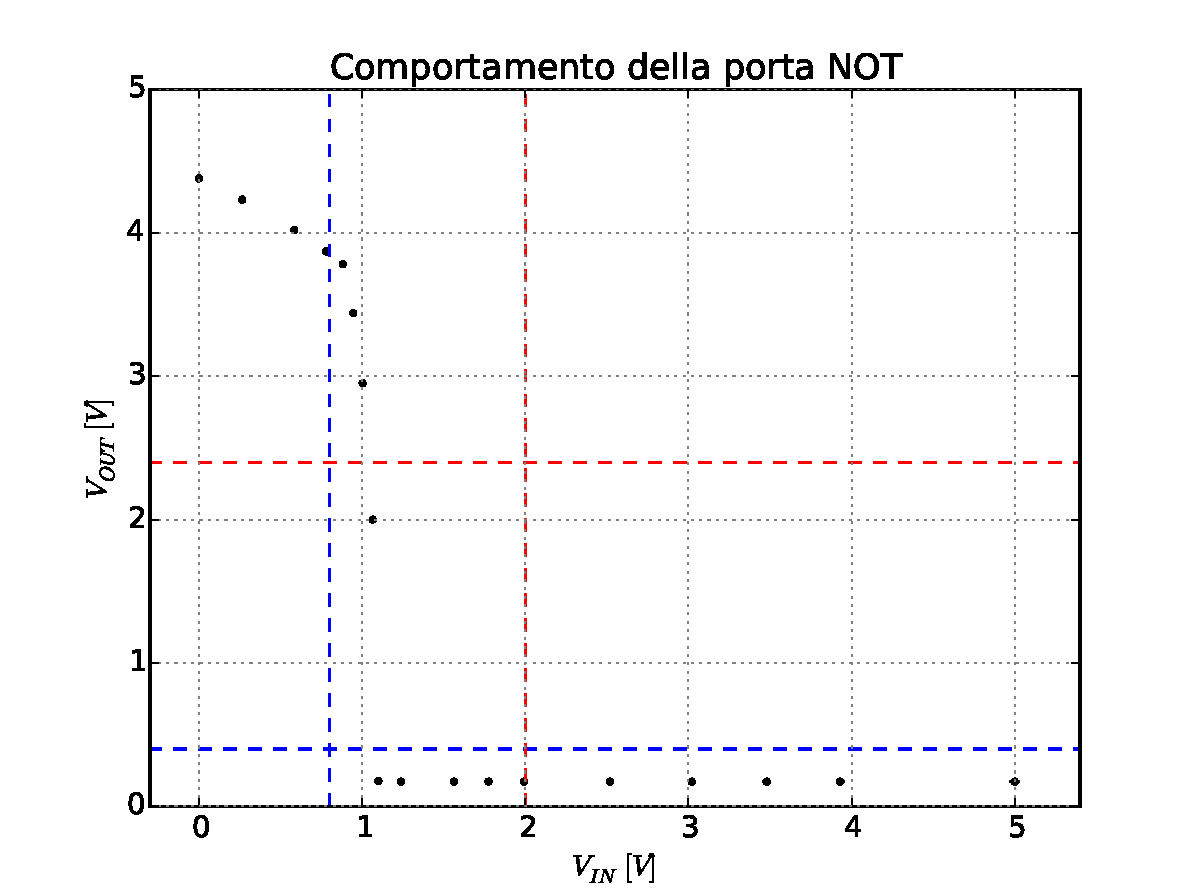
\includegraphics[scale=0.80]{in-ot.pdf}
		\caption{Tensioni operative del NOT}
		\label{f:i1}
	\end{figure}
\end{center}


\subsection{Misura delle correnti e stima del fanout}
\paragraph{Correnti in ingresso} 
Avendo assunto che la corrente in ingresso alla porta logica dipenda dallo stato di funzionamento (ingresso alto o ingresso basso) si è andati a imporre un segnale di $V_{IH} = \SI{4.73\pm 0.03}{\volt}$ osservando una corrente $I_{IH} \lesssim \SI{0.5}{\micro \ampere}$ (si è scelto di usare il multimetro analogico come amperometro per la misura di $I_I$, dal momento che quest'ultimo è in grado di misurare correnti più basse, ma $I_{IH}$ resta troppo piccola per poter essere misurata, con uno spostamento dallo zero inferiore alla mezza tacca con il fondo scala più basso disponibile).

Analogamente per la misura di  $I_{IL}$ si è posta una tensione in ingresso $V_{IL} =$ \SI{152.5(1)}{\milli\volt} rilevando una corrente di $I_{IL}=\SI{-25(1)}{\micro \ampere}$. Si sono considerate positive le correnti entranti nella porta logica e negative quelle uscenti.

Al variare della tensione in ingresso $V_{I}$, rimanendo entro il rispettivo range di funzionamento per ingresso alto o basso, le correnti rilevate non cambiano significativamente. Tali valori sono ampiamente entro i valori massimi riportati dal datasheet.
Come ci aspettiamo per porte realizzate con	logica TTL, le correnti a linea bassa sono molto più alte di quelle a linea	alta.

\paragraph{Correnti in uscita} Si è proceduto dunque alla misura delle correnti in uscita $I_{OL}$ ed $I_{OH}$, rispettivamente quelle rilevate in uscita alla porta logica per lo stato di output basso ed output alto.
Si è quindi montato il circuito in \figurename{ \ref{f:c2}}.

\begin{figure}[H]
	\begin{minipage}{0.7\textwidth}
		\centering
		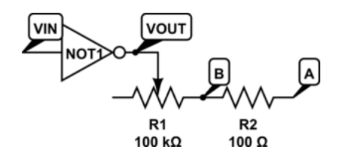
\includegraphics[scale=0.75]{cir2.png}
		\caption{Circuito impiegato per la misurazione di $I_{OL}$ e $I_{OH}$. }
		\label{f:c2}
	\end{minipage}
	\begin{minipage}{0.3\textwidth}
		\begin{tabular}{l}
		$R_{2} = \SI{100.8 \pm 1.1}{\ohm}$\\
		$R_{1} = \SI{94.0 \pm 0.9 }{ \kilo \ohm}$
		\end{tabular}
	\end{minipage}
\end{figure}

Per ottenere le correnti in uscita si è misurata la caduta di potenziale  $V_2$ ai capi di $R_{2}$ con il multimetro digitale; per effettuare le misure di $I_{OL}$ si sono posti $V_{in}$ e $V_A$ alla tensione di alimentazione $V_{CC}=$\SI{5.01 \pm 0.04}{\volt}, mentre per $I_{OH}$ si sono poste le tensioni precedenti a terra. La convenzione sui segni è la
stessa della misura della corrente in ingresso: le correnti entranti
nel dispositivo sono positive, quelle uscenti negative.

Si osserva in entrambi i casi come al variare della resistenza del
potenziometro la corrente vari dapprima lentamente per poi aumentare
bruscamente (supponiamo al raggiungimento dei limiti del dispositivo) quando
la tensione in uscita si discosta dall'intervallo di
corretto funzionamento.

Le misure raccolte sono riportate in appendice in \tablename{ \ref{t:iout}}.

La porta logica sembra dunque non poter essere utilizzata correttamente con
uscita bassa per correnti $I_{OL} \lesssim \SI{5.5}{\mA}$, mentre
ad uscita alta la situazione è meno chiara: sebbene l'uscita sia
ragionevolmente stabile al variare del carico solo al di sotto di
$\sim \SI{0.3}{\mA}$, $V_{out}$ resta entro valori tipici fino a correnti
di qualche \si{\mA}, ed è sufficientemente alta da essere riconosciuta
come tale in ingresso a porte logiche con simili caratteristiche\footnote{il
datasheet dell'integrato da noi analizzato richiede una tensione alta in
input di almeno \SI{2}{\V}, ma come mostrato nella sezione precedente il
dispositivo è in realtà ben più generoso} fino ad oltre la decina di \si{\mA}.
Ci attendiamo comunque che in tali condizioni la porta logica possa essere
instabile, ed è certamente molto sensibile a piccole variazioni del
carico, dunque un limite di corretto funzionamento si dovrà attestare
su valori di $I_{OH}$ non maggiori di pochi \si{\mA}.

Tali stime risultano migliori dei valori limite riportati dal datasheet;
ciò è probabilmente dovuto alla necessità del produttore di avere un certo
margine d'errore, ma è anche possibile che la discrepanza sia imputabile
alla minor severità delle condizioni di test: nel valutare le correnti in
uscita si sono infatti mantenute sia $V_{cc}$ che $V_{in}$ lontane dai
valori limite ammessi dall'integrato, ed è plausibile che avvicinandovisi
il dispositivo sia meno tollerante nelle correnti erogabili.

Con una corrente in ingresso che non supera (in modulo) i \SI{25}{\uA} ed
una corrente erogabile certamente non inferiore a \SI{0.3}{\mA},
una singola porta può fornire il proprio output in ingresso ad una dozzina
di porte simili senza manifestare problemi.

Questo è tuttavia un limite inferiore erroneamente basso: se teniamo conto
del fatto che \SI{25}{\uA} assorbiti corrispondono ad un ingresso basso e ad uscita bassa, la porta è certamente
in grado di	erogare fino a $\sim \SI{5.5}{\mA}$; il fanout è di centinaia
di porte in questa configurazione. 

Analogamente, confrontando la corrente
emessa ad ingresso alto ($\lesssim \SI{0.5}{\micro \ampere}$) con la
corrente sopportabile ad uscita alta ($ > \SI{0.3}{\mA}$) otteniamo un
fanout non inferiore alle 600 porte (ma probabilmente sensibilmente
maggiore).

Prendendo il minore dei due come fanout effettivo della porta,
dovrebbe dunque essere possibile utilizzare una singola porta per
controllarne altre 220.

\section{Montaggio Arduino}
Per la verifica delle caratteristiche dinamiche della porta NOT si è montato un circuito generatore di onde quadre, basato su di un microcontrollore Arduino. 

Si riporta lo schema circuitale in \figurename{ \ref{f:impulsatore}}. 

\begin{figure}[H]
	\begin{minipage}{0.7\textwidth}
		\centering
		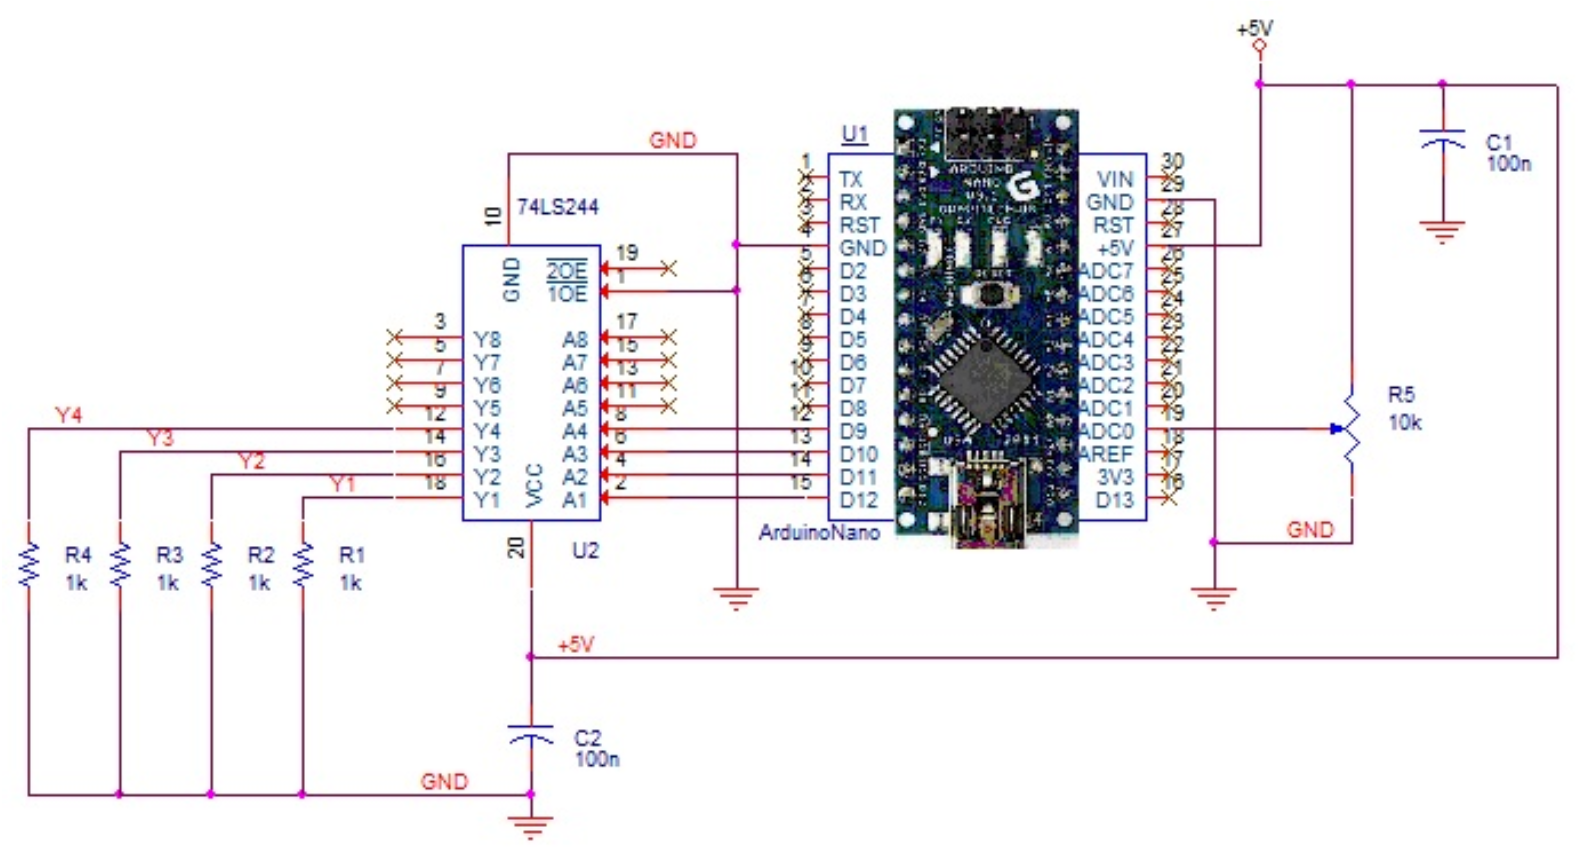
\includegraphics[scale=0.27]{imp.png}
		\caption{Schema del circuito montato}
		\label{f:impulsatore}
	\end{minipage}
	\begin{minipage}{0.3\textwidth}
		\begin{tabular}{l}
			$R_{1}=$\SI{984 \pm 8}{\ohm} \\$R_{2}=$\SI{984 \pm 8}{\ohm} \\$R_{3}=$\SI{982 \pm 8}{\ohm} \\
			$R_{4}=$\SI{983 \pm 8}{\ohm} \\$R_{5}=$\SI{10.2 \pm 0.8}{\kilo \ohm} \\
		$C_{1}=$\SI{114 \pm 6}{\nano\farad} \\$C_{2}=$\SI{114  \pm 6}{\nano\farad}
		\end{tabular}
	\end{minipage}
\end{figure}

Il circuito montato genera delle onde quadre sfasate di $\pi/2$ tra i terminali Y1 e Y2, di frequenza regolabile attraverso il valore del trimmer $R_{5}$, compresa tra pochi \si{\hertz} e \SI{50}{\kilo\hertz}.
In \figurename{ \ref{f:oscil}} si riporta il comportamento osservato ai due terminali.

\begin{figure}[htb]
	\centering
	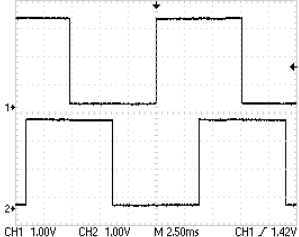
\includegraphics[scale=0.80]{ondaquadra_esempio.png}
	\caption{Comportamento del circuito montato}
	\label{f:oscil}
\end{figure}

Si è verificato che lo sfasamento tra le due onde fosse quello atteso: si è misurato un $\Delta t=\SI{248 \pm 2}{\micro\second}$ tra i fronti di salita dei due canali, a fronte di una frequenza $f=\SI{1.007 \pm 0.001}{\kilo \hertz}$ segue $\Delta \phi=\SI{1.57 \pm 0.01 }{\radian}$, compatibile con $\pi/2$.
\section{Caratteristiche dinamiche}
SI vogliono studiare le caratteristiche dinamiche della porta NOT, per farlo si è inviata all'ingresso della stessa un' onda quadra (generata dalla scheda Arduino, configurata come al punto precedente) di frequenza  $f\sim$\SI{1}{\kilo \hertz} e tensione picco picco $V=$\SI{3.40 \pm 0.20}{\volt}.

\subsection{Tempi di propagazione}
Si è misurato il tempo $\Delta t_{PHL}$ che intercorre tra il centro del fronte di discesa all'ingresso e il centro del fronte di salita sull'uscita. Si è poi ripetuta la misura per $\Delta t_{PLH}$: il passaggio dal fronte di discesa (input) al fronte di salita (output).
Per determinare il centro dei fronti di salita/discesa si è preso il punto in cui i segnali assumevano la metà del loro valore HIGH, ignorando quindi la presenza di overshoot e undershoot, visibili in \figurename{ \ref{f:ripple}}.

\begin{figure}[H]
	\centering
	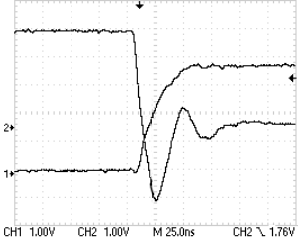
\includegraphics[scale=1]{undershoot_lh.png}
	\caption{Undershoot del segnale in uscita}
	\label{f:ripple}
\end{figure}
\noindent Per la misura si è scelta la scala che ottimizzava la risoluzione, ottenendo:
$$\Delta t_{PHL}=\SI{9.6(6)}{\nano \second} \qquad \text{e} \qquad \Delta t_{PLH}=\SI{14.8(6)}{\nano \second}$$
tali valori risultano in accordo con i valori attesi dal datasheet, che sostiene che entrambi i parametri debbano essere minori di \SI{15}{\nano \second}.

\subsection{Tempi di salita e discesa}
Si sono misurati i tempi di salita $\Delta t^{\uparrow}$ e discesa $\Delta t^{\downarrow}$ del segnale tra il $10 \% $ e il $90 \% $ del valore HIGH, sia in ingresso che in uscita. Si è ottenuto:
$$ \Delta t_{in}^{\uparrow}=\SI{12.2(6)}{\nano \second} \qquad \Delta t_{in}^{\downarrow}=\SI{6.4(6)}{\nano \second} $$
$$ \Delta t_{out}^{\uparrow}=\SI{16.4(6)}{\nano \second} \qquad \Delta t_{out}^{\downarrow}=\SI{48.8(1)}{\nano \second}.$$

\newpage
\section{Appendice}
\begin{table}[hb]
	\centering
	\begin{tabular}{S S}
		\toprule
		$V_{in} [\si{\volt}]$ & 	$V_{out} [\si{\volt}]$\\
		\midrule
		0.000	\pm 0.001    & 4.38 \pm 0.02\\
		0.265 \pm 0.002 & 4.23 \pm 0.02\\
		0.584 \pm 0.003 & 4.02 \pm 0.02\\
		0.780 \pm 0.004 & 3.87 \pm 0.02\\
		0.881 \pm 0.005 & 3.78 \pm 0.02\\
		0.945 \pm 0.005 & 3.44 \pm 0.02\\
		1.003 \pm 0.005 & 2.95 \pm 0.02\\
		1.065 \pm 0.006 & 2.01 \pm 0.01\\
		1.103 \pm 0.008 & 0.1773 \pm 0.009\\
		1.238 \pm 0.009 & 0.1728 \pm 0.009\\
		1.56 \pm 0.01 & 0.1728 \pm 0.009\\
		1.775 \pm 0.02 & 0.1728 \pm 0.009\\
		1.991 \pm 0.02 & 0.1727 \pm 0.009\\
		2.52 \pm 0.02 & 0.1727 \pm 0.009\\
		3.02 \pm 0.02 & 0.1726 \pm 0.009\\
		3.48 \pm 0.02 & 0.1726 \pm 0.009\\
		3.93 \pm 0.02 & 0.1726 \pm 0.009\\
		5.00 \pm 0.03 & 0.1726 \pm 0.009\\
		\bottomrule
	\end{tabular}
	\caption{Comportamento in tensione della porta NOT}
	\label{t:1}
\end{table}

\begin{table}[h]
	\centering
	\begin{tabular}{SS cc SS}
		\toprule
		\multicolumn{2}{c}{Output LOW} &&& \multicolumn{2}{c}{Output HIGH} \\
		\cmidrule{1-2} \cmidrule{5-6}
		{$I_{OL}$ [\si{\mA}]}	& {$V_{out}$ [\si{\V}]}	&&& {$I_{OH}$ [\si{\mA}]}	& {$V_{out}$ [\si{\V}]} \\
		\midrule
		0.0506 (12)	&	0.1758 (10)	&&&	-0.0437 (12)	&	4.12 (3)	\\
		0.2679 (23)	&	0.1868 (10)	&&&	-0.0873 (14)	&	3.93 (3)	\\
		0.328 (3)	&	0.1904 (11)	&&&	-0.1270 (16)	&	3.77 (3)	\\
		1.553 (9)	&	0.2330 (22)	&&&	-0.1637 (18)	&	3.63 (3)	\\
		2.897 (24)	&	0.2660 (23)	&&&	-0.2937 (25)	&	3.53 (3)	\\
		5.21 (4)	&	0.320 (3)	&&&	-3.77 (3)	&	3.28 (3)	\\
		24.01 (22)	&	1.891 (10)	&&&	-13.31 (8)	&	2.300 (21)	\\
		27.88 (24)	&	1.988 (11)	&&&	-16.91 (9)	&	1.860 (10)	\\
		\bottomrule
	\end{tabular}
	\caption{Comportamento in corrente della porta NOT}
	\label{t:iout}
\end{table}
\end{document}
